\chapter{Datenquelle 2: EASA und Easy Access Rules}

    \section{European Union Aviation Safety Agency}

\begin{quote}
\textcolor{red}{Einführung zur EASA. Neue Position und Bedeutung für den Prozess. Was sind Easy Access Rules und welche Bedeutung haben sie für uns. Hard law / Soft law. Added benefit durch AMC/GM}
\end{quote}
\begin{quote}
\textcolor{green}{1-2 Seiten}
\end{quote}

        
        \subsection{Bedeutung nach VO 2023/1768ff.}
        
        \pagebreak
        \subsection{Easy Access Rules}

Im Rahmen der behandelten Definitionen aus der Studie zu funktionalen Anforderungen bibliografischer Datensätze \acs{FRBR} (siehe \ref{frbr}) bilden die \textit{Easy Access Rules} eine weitere \textit{Manifestation} des bestehenden \textit{Werkes} der referenzierten, abgedeckten Verordnung.
Auch wenn die \ac{EAR} den Umfang bestehender \textit{Manifestationen} inhaltlich um \textit{Annehmbare Nachweisverfahren} und \textit{Guidance Material} erweitern, so ändern sie nicht 



\begin{quote}
\textcolor{green}{\~1.5 Seiten}
\end{quote}

        \pagebreak
        \subsection{Annehmbare Nachweisverfahren}

        Die \ac{EASA} ist nach der Anforderung \textsf{ATM/ANS.AR.A.015.a} angehalten, annehmbare Nachweisverfahren (engl. Accepted Means of Compliance (AMC)) zu entwickeln, welche zur Bewertung der Compliance herangezogen werden können und dessen Abdeckung eine vollständige Abdeckung der zugrundeliegenden einschlägigen Verordnung garantiert. 
        \cite[Anh. II]{2017R0373}


    \subsubsection{Alternative Nachweisverfahren}
        
        

\subsection{Guidance Material}

\begin{quote}
\textcolor{green}{\~0.5 Seiten}
\end{quote}
        \pagebreak
    \section{EASA eRules Plattform}

    Die \ac{EASA} eRules Plattform ist ,,einheitliche, einfach zugängliche, online Datenbank für alle in der Luftfahrt anwendbaren Regeln für Stakeholder im europäischen Luftraum``.
    \cite[5]{easa_xml_doc}

    Als ein Produkt dieser Plattform werden die sogenannten Easy Access Rules definiert und bis dato (24.6.22) in zwei Formaten veröffentlicht. 

    
Am 26. Januar 2023 veröffentlichte die EASA die Entscheidung, Easy Access Rules fortan auch in einem maschinenlesbaren XML Format Endnutzern bereitzustellen. \cite{easa_xml_publication}


\subsection{Informationsarchitektur}
\label{ch:easa_arch}

    Im Rahmen der eRules Plattform und des maschinenlesbaren \ac{XML} Formates, werden Inhalte in kleine sogenannte ,,Topics`` unterteilt.
    Ein Topic repräsentiert eine \ac{EU} Durchführungsbestimmung (siehe \ref{ch:ir}); eine \ac{EU} Delegierte Bestimmung; ein Annehmbares Nachweisverfahren der \ac{EASA}; \ac{EASA} Guidance Material; oder sog. \ac{EASA} \acf{CertS}\footnote{(CS) wegen Überschneidung mit \acf{CS} geändert}. \cite[S. 5f]{easa_xml_doc}
    
Topics werden repräsentativ ihrer konzeptuellen Beziehungen zwischen den unterschiedlichen Topics in der baumartigen Struktur abgebildet.
Hierbei werden Topics, welche Verordnungen oder \ac{CertS} abbilden meist auf einem strukturell höheren Level und alle diesem zugeordneten Topics wie. \acsp{AMC}, \acsp{GM}, oder anderen Gesetzesgrundlagen dargestellt.


        
        \subsubsection{Publikationsformat}

    Die für die Publikation der maschinenlesbaren Dokumente wählte die \ac{EASA} die von \acf{MS} etablierte und standardisierte \acf{OPC}\footnote{\acs{ECMA}-376, ISO/IEC 29500-2}.
    Dieser Standard ist Teil der Familie an \ac{XML} Schemata, welche gemeinsam als \acf{OOXML} bezeichnet werden\footnote{ ISO/IEC 29500} und \ac{XML} Semantiken für Textverarbeitungs-, Tabellen\-kal\-ku\-lations- und Präsentationsdokumente -- oder hiermit konformen Dokumenten -- bereitstellen. 
    \cite[vii]{easa_opc_iso} 
    Die Besonderheit dieses Formates ist es, dass das Gesamtdokument in kleineren Parts\footnote{gemäß 6.2 ISO/IEC 29500-2 \cite{easa_opc_iso}} strukturiert wird, welche nach der Definition der \ac{OPC} -- ähnlich wie ein Archiv -- in ein Gesamtdokument zusammengefasst werden.
    Hierauf basierende Standards, wie \ac{OOXML}, definieren meist nur die Struktur einzelner Parts, was eine konforme Erweiterung des Gesamtdokumentes durch weitere Parts problemlos ermöglicht.   
    Dies bedeutet unter anderem, dass valide Dokumente Teil von größeren Gesamtdokumentes sein können, wessen weitere Parts keinen Einfluss auf dessen Benutzung als konformes Open Office-Dokument nehmen.
    Genau von dieser Eigenschaft hat die \ac{EASA} Gebrauch gemacht und ihre Informationen auf zwei Arten in das Gesamtdokument integriert:

            \subsubsection{Anforderungsinhalte}

    Inhalte von Topics werden unter Release 1.0.0 der eRules \ac{XML} Spezifikation als ,,opaque data structure`` angesehen.
    Dies bedeutet, dass im Zug dieses Releases keine inhaltliche Struktur der Inhalte der Topics definiert wurde.
    Es bleibt jedoch den Anwender:innen überlassen, Implementationen auf die Angaben innerhalb des beschriebenen \acs{OOXML} Formates zu stützen.
    \cite[6]{easa_xml_doc}

    % \medskip
    Nach diesem Standard sind die textuellen Inhalte der einzelnen Topics Teil des Textverarbeitungsdokumentes\footnote{Part Name: "\textit{/word/document.xml}"} und lassen sich damit auch über eine grafische Textbearbeitungsoberfläche (bspw. \ac{MS} Word) einsehen und bearbeiten.
    Hierbei werden Textinhalte des Dokumentes so strukturiert, dass die einzelnen Entitäten voneinander isoliert und über eine -- innerhalb des Dokumentes -- lokal einzigartige ID, eindeutig identifizierbar gemacht werden.
    So können die Inhalte bei Bedarf beliebig bearbeitet werden, ohne die Struktur der Topics oder die Integrität anderer strukturellen Verweise zu gefährden.
            % Außerdem ist es so möglich, Einträge in den Metadaten auf die entsprechenden Anforderungsinhalte verweisen zu lassen. 

            \subsubsection{Metadaten}

    % Zusätzlich zu den Inhalten ermöglicht es der \ac{OOXML} Standard, weitere Parts an das Textdokument anzuhängen.
    Die \ac{EASA} nutzt zusätzlich die Möglichkeit, konforme \ac{OOXML} um eigene Parts zu erweitern, um das inhaltliche Dokument mit Metadaten der einzelnen Topics, auf Basis des internen \ac{EASA} \ac{CCMS}, zu bereichern.
    Diese Metadaten enthalten interne Informationen zu der Struktur des Dokumentes und den einzelnen Anforderungen und stehen dem Endnutzer in Form eines \ac{OPC} Parts  zur Verfügung.
    Dessen Struktur beruht auf einem eigenen \ac{XML} Schema, welches in der entsprechenden Dokumentation der \ac{EASA} definiert ist.

\pagebreak
\subsection{Analyse der Metadaten}

    Die für diese Analyse relevanten Attribute, welche Metadaten der oben definierten Topics beschreiben, werden im Rahmen der Dokumentation unter der Gruppe ,,\textsf{topic-metadata}``\footnote{\ac{XSL} Attribute Group} festgehalten.
    Diese Gruppe beinhaltet die im Folgenden analysierte Attribute.\footnote{Alle beschriebenen Attribute werden durch den Typ String ohne jegliche Einschränkungen abgebildet und im Folgenden durch ,,[AttributName] Attribut`` oder -- gemäß dem XPath Standard -- ,,@[AttributName]`` referenziert} \cite[9]{easa_xml_schema}

    \subsubsection{ERulesId}

Die \textit{ERulesId} stellt eine -- über alle publizierten Dokumente hinweg -- einzigartige Kennung eines jeden Topics dar.
Dies ermöglicht eine einfache, einheitliche Referenzierung von Topics unabhängig von deren zugehörigem Dokument.
Die \ac{EASA} garantiert diesbezüglich, dass die Id über den gesamten Lifecycle des Topics unveränderlich sind. \cite[17]{easa_xml_doc}

In Bezug auf die Impactanalyse, bietet dieses Attribut einen großen Vorteil, da die definierten Anforderungen an eine \textit{Eindeutige Kennung} (vgl. \ref{model_anforderungen}) bereits für alle Topics der \ac{EASA}\footnote{Darunter, durch \ac{IR}, auch \atmans Anforderungen} erfüllt sind.
% \medskip
\begin{quote}
Beispiel:
\textsf{ERulesId="{}ERULES-1891294191-107"}
\end{quote}

% A unique identifier attribute for every topic in the exported XML file, which allows the unique identification of a topic across all the exported XML files from EASA. The ERulesId value is unchanged: • from publication to publication, everywhere the topic is reused; and • from version to version, throughout the entire life cycle of the topic.  
    
    \subsubsection{Domain / Activity Type}

Die \textit{Domain} und der \textit{Activity Type} eines Topics bezeichnen dessen Aufgabenbereich sowie die technische Beschreibung der darin vollbrachten Aufgabe \cite[S. 18]{easa_xml_doc}.
Im Umfang der nach \vo{VO}{EU}{2018/1139} i.V.m. \vo{VO}{EU}{628/2013} definierten Aufgabenbereiche kann in unserem Falle immer die \textit{Domain} \atmans angenommen werden.

Mögliche Werte des \textit{ActivityType}-Attributs beinhalten u.a.\footnote{Nicht holistische Liste an Beispielen \cite[vgl.][S.18 -- 19]{easa_xml_doc}} die unter \atmans definierten Aufgaben (siehe \ref{beg:atmans}).
Sie geben in der folgenden Analyse Auskunft darüber, für welche \atmans Ausrüstungen die Topics eine Relevanz aufweisen.
Dies kann u.a. genutzt werden, um die Relevanz neuer Anforderungen zu ermitteln oder irrelevante Anforderungen im Nachweisführungsprozess anderer Ausrüstungen auszuschließen.  

\begin{quote}
    Beispiel:
    \textsf{ActivityType="Meteorological Services (MET)"}
\end{quote}
   
    \subsubsection{AircraftCategory / AircraftUse / RegistryState}

Die Attribute \textit{AircraftCategory}, \textit{AircraftUse} und \textit{RegistryState} beziehen sich auf die Klassifizierung und Zuordnung von Anforderungen an Flugzeuge und haben für \atmans Equipment kein Gewicht\footnote{Eine vorangehende Analyse hat ergeben, dass diese Attribute in den \atmans Dokumenten nicht verwendet werden}. \cite[20, 21, 26]{easa_xml_doc}
    
    \subsubsection{AmendedBy}

Im Falle von Änderungen des \textit{Topics} referenziert dieses Attribut die lokale Konsolidierung der \ac{EAR}
\cite[21]{easa_xml_doc}.
Nach deren Publikation unbearbeitete \textit{Topics} führen den Wert \textsf{"{}Initial issue;"}

\begin{quote}
    Beispiel:
    \textsf{AmendedBy="{}Amendment 1;"}\footnote{Die Kennung der Änderung bezieht sich ausschließlich auf die aktuelle \ac{EAR}}
\end{quote}
    
    \subsubsection{ApplicabilityDate / EntryIntoForceDate }

Die Attribute \textit{Applicability-} und \textit{EntryIntoForceDate} beschreiben im Falle von Topics, welche sich auf Durchführungsbestimmungen beziehen, den entsprechenden zeitlichen Rahmen von deren Gültigkeit.
Das \textit{ApplicabilityDate} repräsentiert dabei -- unabhängig von dem juristischen Wortlaut -- den letzten Tag der Übergangsperiode. 
Das \textit{EntryIntoForceDate} hingegen repräsentiert das offizielle Inkrafttreten rechtlicher Durchführungsbestimmungen, nach welcher die rechtliche Bindung der in dem Topic abgebildeten Anforderung beginnt.
\cite[21]{easa_xml_doc}
Mangels rechtliche Bindung verfügen Topics in Bezug auf \acsp{AMC} oder \ac{GM} nicht über diese Attribute.\footnote{Strukturell sind alle Topics gleich, der Wert bleibt lediglich leer}
    
    \subsubsection{EquivalentForeignRegulation}

Das Attribut \textit{EquivalentForeignRegulation} äquivalente Regularien von nicht \ac{EU} Mitgliedstaaten.
Diese Informationen werden -- nach Angaben der \ac{EASA} -- hauptsächlich zum Angleichen von Designstandards von Flugzeugdesigns genutzt \cite[22]{easa_xml_doc}, finden nach eigener Auswertung aber auch im \atmans Sektor Anwendung, um bspw. international gemeinschaftliche Nachweisverfahren zur Luftdatenverarbeitung zu etablieren (siehe Beispiel).

\begin{quote}
    Beispiel:
    \textsf{EquivalentForeignRegulation="{}AC No: 20-153B;"}\footnote{Referenziert \ac{FAA}: \ac{AC} 20-153B - ,,Acceptance of Aeronautical Data Processes and Associated Databases``}$^,$\footnote{Semikolon beschreibt mögliche Auflistung mehrerer (durch Semikola getrennte) Einträge }
\end{quote}

    \subsubsection{ICAOReference}

Verweist auf -- im Rahmen des \textit{Topics} -- relevante \ac{ICAO} \acp{SARP}. 
\cite[23]{easa_xml_doc}

\begin{quote}
    Beispiel:
    \textsf{ICAOReference="{}Annex 11; Annex 19;"}
\end{quote}
    
    \subsubsection{Keywords}

    Die Verwendung des \textit{Keyword} Attributs ist nach der offiziellen Dokumentation nicht genau festgelegt.
    Es wird verwendet, um weitere Metadaten anzuhängen oder eine Kategorisierung anhand einzelner Schlüsselwörter umzusetzen.
\cite[23--26]{easa_xml_doc}
    \begin{quote}
    Beispiel:
    \textsf{Keywords="{}Safety measures; safety tracking"}
\end{quote}

    \subsubsection{RegulatedEntity}

Die regulierte juristische Person (\textit{regulated entity}) definiert, an wen die -- im \textit{Topic} definierte -- Anforderung gerichtet ist und wer diese im gleichen Zug zu erfüllen hat.
Diese \textit{Entities} beschreiben entweder Stakeholder:innen der Luftfahrtindustrie oder der zuständigen Behörde\footnote{hier \ac{EASA}} \cite[26]{easa_xml_doc}.

Im Rahmen der \atmans Anforderungen kann dieses Attribut auch die Anbieter der definierten \atmans Dienste definieren.
Diese Informationen können so eine sehr gute Abbildung erzeugen, welche Bereiche im \atmans Sektor von entsprechende \textit{Topics} reguliert werden.  
    \begin{quote}
    Beispiel:
    \textsf{RegulatedEntity="{}ATS provider; ANS provider;"}
\end{quote}

    
    \subsubsection{Regulatory Source}

Die Funktion dieses Attribut beschreibt -- analog zur Definition aus \ref{model_anforderungen} -- die Regulatorische Quelle der Durchführungsrichtlinie.
Im Genaueren definiert die \textit{Regulatory Source} den Rechtsakt, welcher das \textit{Topic} eingeführt\footnote{i.V.m. \textit{@AmendedBy} \textsf{"{}InitialIssue"} / "FurtherIssue"} oder zuletzt konsolidiert\footnote{i.V.m. \textit{@AmendedBy} \textsf{"{}Amendment [...]"}} hat \cite[27]{easa_xml_doc}. 

    \begin{quote}
    Beispiel:
    \textsf{RegulatorySource="{}Regulation (EU) 2021/1338"}
\end{quote}

    \subsubsection{Regulatory Subject}

Der Regulierungsgegenstand (\textit{Regulatory Subject}) referenziert das relevante Material des \textit{Topics}. 
Dieses beschreibt den strukturellen Teil, in welchem es durch das Amtsblatt oder die \ac{EASA} Website publiziert wurde \cite[28]{easa_xml_doc}.
Im Falle der \atmans Anforderungen aus der \vo{DVO}{EU}{2017/373} bezieht sich dieses Attribut entweder auf den eigenen Verordnungstext\footnote{Wert ,,cover regulation``} oder einer der, in den Anhängen, definierten ,,Parts``.
\begin{quote}
    Beispiel:
    \textsf{RegulatorySubject="Part-ATS;"}
\end{quote}


    \subsubsection{TechnicalSubjectMatter / EASACategory}

Referenziert zumeist technische Systeme von Flughäfen oder \ac{EASA} Kategorisierungen von Landebahnen und findet für \atmans Equipment keine Anwendung. \cite[28--29, 31]{easa_xml_doc} 

   \pagebreak
    \subsubsection{TypeOfContent}

Das \textit{TypeOfContent} Attribut definiert den Typ und die Funktion des \textit{Topics}.
Neben den oben definierten Typen von \textit{Topics} spezifiziert das Attribut im Falle von untergeordneten Topics auch den Typen des nächsthöheren, referenzierten \textit{Topics} 
(bspw.: ,,AMC to IR``\footnote{Annehmbare Nachweisverfahren von Anforderungen}, ,,GM to AMC``\footnote{Anleitungen zu Annehmbaren Nachweisverfahren}, ,,GM to IR``\footnote{Anleitungen zu Anfoderungen})

    \begin{quote}
    Beispiel:
    \textsf{TypeOfContent=\\"{}AMC to IR (Acceptable means of compliance to implementing rule);"}
\end{quote}

    
    \subsubsection{ParentIR}

    Das \textit{ParentIR} Attribut referenziert\footnote{durch das Titel-Attribut (@source-title) des anderen Topics (nicht Teil von topic-metadata)} das jeweils -- nach der Table Of Content (ToC) Hierarchie -- direkt-übergeordnete \textit{Topic}.
    Befindet sich das Topic bereits auf der obersten Ebene, bleibt dieses Feld leer.
    Diese Eigenschaft ermöglicht es, die Position eines \textit{Topics} innerhalb der Hierarchie zu bestimmen und im Falle eines \ac{AMC} oder \ac{GM} \textit{Topics} die jeweils abgedeckte Grundlage zu bestimmen.
    Wie in der Abbildung \ref{fig:parent_ir} dargestellt, referenzieren alle untergeordneten \textit{Topics} durch dieses Attribut das jeweils übergeordnete. 

    \begin{figure}[h]
        \centering
        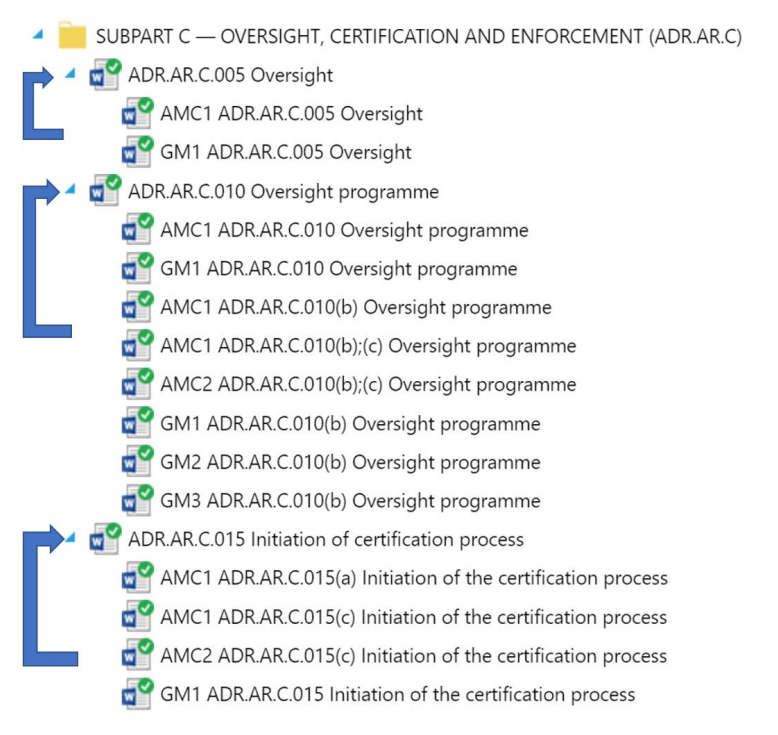
\includegraphics[width=0.75\linewidth]{gfx/parentir.png}
        \caption{Referenzierung des @ParentIR Attributs }\cite[31]{easa_xml_doc}
        \label{fig:parent_ir}
    \end{figure}

    

    % \subsection{Vor- \& Nachteile}
    \pagebreak
    \section{Bewertung der Datenquelle}

    Die \acf{EASA} stellt der Öffentlichkeit -- auf Basis ihrer definierten Aufgaben -- \textit{annehmbare Nachweisverfahren} und \textit{Guidance Material} zur Verfügung.
    Diese werden im Weiteren zusammen mit den entsprechenden Durchführungsbestimmungen in der Form von \acf{EAR} veröffentlicht. 
    Um die Integration ihrer Daten fortlaufend zu stärken, ist die \ac{EASA} bemüht, nützliche Informationen Nutzer:innen in zugänglichen und maschinenlesbaren Formaten bereitzustellen. 

    Das publizierte Datenschema (Version 1.0.0) in Kombination mit den maschinenlesbaren Daten der \acp{EAR} ermöglicht Nutzer:innen einen Zugang zu den internen Metadaten der \ac{EASA} zu sämtlichen ihrer Publikationen.
    Diese analysierte Datenquelle ermöglicht es ebenfalls Inhalte auf die verfügbaren Metadaten referenzieren zu können.


    Die große Schwachstelle dieser Datenquelle besteht in dessen Verfügbarkeit.
    Die \ac{EASA} kuriert folglich nur ausgewählte Durchführungsbestimmungen und publiziert nach Entwicklung oder der Anpassung entsprechender \textit{Annehmbaren Nachweisverfahren} und \textit{Guidance Materials} dessen neue Version für alle Nutzer:innen.
    \footnote{Zum aktuellen Zeitpunkt (02/2024) wurden die Änderungen der \vo{DVO}{EU}{2023/1771} bzgl. der \vo{DVO}{EU}{2017/373} aus 09/2023 noch nicht auf die entsprechende \ac{EAR} (Easy Access Rule for \atmans) übertragen.}
     